\chapter{Talen en Berekenbaarheid}\label{berekenbaarheid}


\section{De Turingmachine als herkenner en beslisser}\label{turingmachines}

In vorige hoofdstukken hebben we twee klassen uit de Chomsky
hi\"erarchie van dichtbij bekeken, met hun bijbehorende herkenners. We
weten al dat reguliere talen contextvrij zijn en dat er talen bestaan
die niet contextvrij zijn. Het is tijd om machinerie op te zetten om
zekere niet-contextvrije talen te herkennen of te beslissen. De
machine die we zullen gebruiken is de Turingmachine: die is
krachtiger dan de LBA die we al eens vermeld hebben. Op de LBA komen
we later nog terug in dit hoofdstuk. 

Ruwweg bestaat een Turingmachine uit een twee-zijdig onbegrensde band
die verdeeld is in vakjes, een controle-eenheid, en een leeskop die op
elk ogenblik de inhoud van een vakje op de band kan lezen. De actie
van de machine hangt af van de inwendige toestand van de
controle-eenheid en het teken onder de leeskop. Figuur~\ref{turing1}
toont die onderdelen en ook de actie beschreven door de $\delta$ van
de Turingmachine.


\begin{figure}[h]
\includegraphics[%
  width=0.6\linewidth,
  keepaspectratio]{turing1}
\caption{Schema van een Turingmachine\label{turing1}}
\end{figure}

\vspace{-5cm}\hspace{10cm}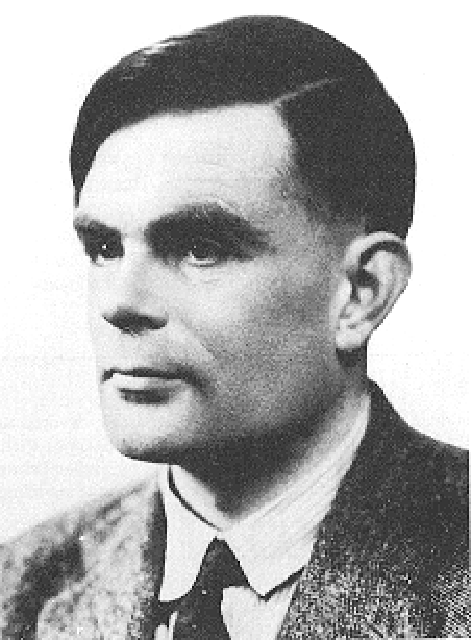
\includegraphics[%
  width=0.2\linewidth,
  keepaspectratio]{afbeeldingen/turing}


Meer formeel:
 \grijs{\begin{definitie} Turingmachine\\
{\rm
Een {\bf Turingmachine} is een 7-tuple
%
$(Q, \Sigma, \Gamma, \delta, q_s, q_a, q_r)$
%
waarbij $Q, \Sigma, \Gamma$ eindige verzamelingen zijn en

\begin{itemize}
\item 
Q is een verzameling toestanden

\item 
$\Sigma$ is een input alfabet dat \# niet bevat

\item 
$\Gamma$ is het tape alfabet; $\# \in \Gamma$ en $\Sigma \subset \Gamma$

\item 
$q_s$ is de starttoestand

\item 
$q_a$ is de accepterende eindtoestand


\item 
$q_r$ is de verwerpende eindtoestand (r van reject) verschillend van $q_a$


\item 
$\delta$ is de transitiefunctie: een totale functie met signatuur

$~~~~~~~~~~Q \times \Gamma \rightarrow Q \times \Gamma \times \{L,R,S\}$

\end{itemize}
}
\end{definitie}
}


De machine wordt ge\"{i}nitialiseerd als volgt:
\begin{itemize}
\item een eindig aantal symbolen uit het input alfabet worden
aaneensluitend op de band gezet: dat is de inputstring; op de rest
komt een \#
\item de machine wordt in toestand $q_s$ gezet
\item de leeskop wordt gepositioneerd op het meest linkse teken van de
inputstring; als de string leeg is, dan op een willekeurig hekje
\end{itemize}


De machine werkt nu als volgt: op basis van het teken onder de
leeskop en de toestand van de machine (dus $Q \times \Gamma$) wordt
met behulp van $\delta$ bepaald naar welke toestand de machine moet
overgaan, welk symbool er moet geschreven worden en welke beweging de
leeskop maakt (dus $Q \times \Gamma \times \{L,R,S\}$). Dit wordt
uitgevoerd en dat blijft zo doorgaan 
\begin{itemize}
\item totdat de machine in $q_a$ komt: de inputstring is geaccepteerd
en eventueel beschouw je wat nu op de band staat als het resultaat
van een berekening
\item totdat de machine in $q_r$ komt: de inputstring is verworpen
\item en blijft zo doorgaan ... de machine zit in een {\em oneindige
lus}
\end{itemize}

We hebben reeds met de Turingmachine kennisgemaakt in een vroegere
cursus, dus moeten we er hier niet heel diep op ingaan. Wel willen we
nog de klassieke varianten van de definitie van Turingmachine
aangeven: eventueel aan jullie om te bewijzen dat die alle {\em
equivalent} zijn (maar je zal zelf een redelijke notie van
equivalentie moeten formaliseren).

\begin{itemize}
\item de leeskop kan enkel naar Links of Rechts, maar niet blijven Staan
\item er is meer dan \'{e}\'{e}n accepterende toestand en/of meer dan
\'{e}\'{e}n verwerpende toestand
\item de band is onbegrensd in slechts \'{e}\'{e}n richting
\item er is meer dan \'{e}\'{e}n band
\item het inputalfabet heeft slechts twee symbolen\label{twosymbols}
\item er zijn slechts drie toestanden
\item de machine heeft twee stacks i.p.v. een oneindige band
\end{itemize}


Tenslotte nog iets over het hekje \#: het wordt o.a. gebruikt om aan
te geven dat een vakje op de band nog niet is beschreven (al mag de
Turingmachine het later wel schrijven). In veel teksten wordt het
beschreven als {\em het blanco symbool} en er wordt het symbool $\sqcup$
voor gebruikt. We zullen soms ook verwijzen naar ons \# met {\em het
blanco symbool}, of het {\em hekje}.


Voor een gegeven Turingmachine TM kunnen we $\Sigma^*$ verdelen in drie
disjuncte stukken:
\begin{enumerate}
\item de strings die door de TM worden geaccepteerd: $L_{TM}$
\item de strings waarvoor de TM niet stopt: $\infty_{TM}$
\item de rest
\end{enumerate}
We gebruiken die verzamelingen in de volgende definities.

% \clearpage
 \grijs{\begin{definitie} Herkennen\\
{\rm
Een Turingmachine TM herkent $L_{TM}$
}
\end{definitie}}


Een aansluitende definitie is natuurlijk

 \grijs{\begin{definitie} Turing-herkenbare taal\\
{\rm
Een taal L is Turing-herkenbaar indien er een Turingmachine TM bestaat
zodanig dat  $L = L_{TM}$
}
\end{definitie}}


Laten we meteen een voorbeeld geven van een herkenbare taal L en een
TM die L herkent: $\Sigma = \{a,b\}$, en $L = \{a\}^*$. De volgende
tabel beschrijft $\delta$:

\begin{table}[ht]
\center
\begin{tabular}{|l|c||l|c|c|}
\hline
$Q$    & $\Gamma$   &  $Q$  &  $\Gamma$ &  LRS \\ \hline
$q_s$  &  a         &  $q_s$&   \#      &  R   \\ 
$q_s$  &  b         &  x    &    b      &  S   \\ 
$q_s$  &  \#        &  $q_a$&    -      &  -   \\ 
x      &  a         &  x    &    a      &  S   \\ 
x      &  b         &  x    &    b      &  S   \\ 
x      &  \#        &  x    &    \#     &  S   \\ 
\hline
\end{tabular}
\caption{TM die $\{a\}^*$ herkent} \label{turing3}
\end{table}
Het is duidelijk dat $\infty_{TM}$ niet leeg is: voor elke string niet
in L gaat de machine in een lus. Voor dezelfde taal L bestaat ook een
TM die altijd stopt, bijvoorbeeld:

\begin{table}[ht]
\center
\begin{tabular}{|l|c||l|c|c|}
\hline
$Q$    & $\Gamma$   &  $Q$  &  $\Gamma$ &  LRS \\ \hline
$q_s$  &  a         &  $q_s$&   \#      &  R   \\ 
$q_s$  &  b         &  $q_r$&    -      &  -   \\ 
$q_s$  &  \#        &  $q_a$&    -      &  -   \\ 
\hline
\end{tabular}
\caption{TM die $\{a\}^*$ beslist} \label{turing4}
\end{table}

Dat onderscheid vatten we in de volgende definities:

 \grijs{\begin{definitie} Beslissen\\
{\rm
Een Turingmachine TM beslist een taal L, als TM L herkent en bovendien
$\infty_{TM} = \emptyset$
}
\end{definitie}}


en

 \grijs{\begin{definitie} Turing-beslisbare taal\\
{\rm
Een taal L heet Turing-beslisbaar als er een Turingmachine is die L
beslist.
}
\end{definitie}}


A priori is het niet duidelijk dat herkennen en beslissen verschillen
van elkaar, maar het zal blijken dat er een belangrijk onderscheid
tussen bestaat. Wat wel duidelijk moet zijn: een beslisbare taal is
ook herkenbaar.


 \grijs{\begin{definitie} Co-herkenbaar/co-beslisbaar\\
\textup{Een taal L is \textbf{co-herkenbaar/co-beslisbaar} als $\overline{L}$
herkenbaar/beslisbaar is.}
\end{definitie}}

 \grijs{\begin{stelling}\label{coherkenbaar}
Als L beslisbaar is, dan is L ook co-beslisbaar.
\end{stelling}}
\begin{proof}
In de Turingmachine die L beslist, verwissel je de rol van $q_a$ en
$q_r$.
\end{proof}

 \grijs{\begin{stelling}
Als L herkenbaar is en co-herkenbaar, dan is L beslisbaar.
\end{stelling}}
\begin{proof}
Laat M1 de machine zijn die L herkent, en M2 de machine die $\overline{L}$
herkent. De idee is nu dat we M1 en M2 samen laten lopen als een
nieuwe machine M, in parallel: zodra M1 accepteert, dan accepteert M,
en zodra M2 accepteert, dan verwerpt M. M1 en M2 kunnen niet samen
accepteren, en voor elke string zal minstens \'{e}\'{e}n van de
machines M1 en M2 stoppen - in zijn aanvaardende toestand. M beslist L.


De bovenstaande constructie van M is informeel en eigenlijk moeten we
die formeler maken. Dat kan door M te defini\"eren als een 2-tape
machine: je kan zelf de details uitwerken.
\end{proof}


\grijs{\begin{stelling}
Er bestaat een taal die niet herkenbaar is.
\end{stelling}}
\begin{proof}
Het bewijs steunt op het begrip kardinaliteit: we weten van vroeger
dat het aantal Turingmachines aftelbaar oneindig is. We weten ook dat
elke Turingmachine juist \'{e}\'{e}n taal herkent\footnote{Zorg dat je
snapt waarom!}. En tenslotte weten we ook dat het aantal talen
niet-aftelbaar oneindig is, want de verzameling talen is ${\cal
P}(\Sigma^*)$. Bijgevolg bestaat een niet-herkenbare taal. In feite
is daarmee zelfs bewezen dat er niet-aftelbaar veel niet-herkenbare
talen bestaan. Meer nog: bijna alle talen zijn niet-herkenbaar!
\end{proof}



Wat zijn we van plan met Turingmachines en die definities ...

\begin{itemize}
\item het onderscheid tussen beslissen en herkennen verder bestuderen
\item reguliere en contextvrije talen in dit plaatje inpassen
\item voorbeelden van talen bekijken die niet-herkenbaar zijn of
niet-beslisbaar
\end{itemize}

De engelse termen zijn:
\begin{itemize}
\item herkenbaar: recognisable en recursive enumerable
\item beslisbaar: decidable en recursive
\end{itemize}
In Sectie~\ref{enumerator} zullen we de historische reden voor de
term {\em enumerable} zien.


\paragraph{Zelf doen:} Wat denk je van de uitspraken:

\begin{itemize}
\item elke string is herkenbaar
\item elke string is beslisbaar
\item elke eindige taal is beslisbaar/herkenbaar
\item de unie/doorsnede van twee herkenbare talen is herkenbaar
\item de doorsnede van een herkenbare en een beslisbare taal is beslisbaar
\end{itemize}




% \clearpage
\section{Grafische voorstelling van een Turingmachine}

Net zoals bij FSA's en PDA's kunnen we een Turingmachine goed
visualiseren met een graaf: daarin zijn de knopen de toestanden van de
TM. Een voorbeeld verduidelijkt veel: Figuur~\ref{turing2} toont de
voorstelling met een graaf van een TM die (hopelijk) de taal
$\{0^n1^n|n \geq 0\}$ beslist.




\begin{figure}[h]
\begin{center}\includegraphics[%
  width=0.7\linewidth,
  keepaspectratio]{turing2}\end{center}
\caption{Grafische voorstelling van een Turingmachine\label{turing2}}
\end{figure}

Vanuit elke toestand vertrekken zoveel bogen als er elementen zijn in
$\Gamma$ (maar sommige worden samengenomen). Het label op een boog
symboliseert de $\delta$ van de machine. Een \_ wordt gebruikt om aan
te duiden dat het er niet toe doet welk symbool er staat: typisch
wanneer het een overgang naar een eindtoestand betreft.

% \clearpage

We kunnen in woorden beschrijven wat die machine doet met een input
van nullen en enen (en ook de lege string).

\begin{itemize}
\item als in de starttoestand een
\begin{itemize}
\item \# gezien wordt, dan accepteer
\item 1 gezien wordt, dan verwerp
\item 0 gezien wordt, veeg die uit en ga rechts naar de toestand $n$ die alle
nullen overslaat
\end{itemize}

\item als in toestand $n$ een
\begin{itemize}
\item \# gezien wordt, verwerp
\item 1 gezien wordt, ga rechts naar $e$ die alle enen overslaat
\item 0 gezien wordt, ga naar rechts
\end{itemize}


\item in toestand $e$
\begin{itemize}
\item zolang 1-en gezien worden, ga naar rechts
\item bij een 0, verwerp
\item bij een \#, ga links naar toestand $v$ die \'{e}\'{e}n 1 zal uitvegen
\end{itemize}

\item in $v$
\begin{itemize}
\item een 0 of \# zijn fout, dus verwerp
\item veeg de 1 uit en ga links naar toestand $l$ die de linkerkant
van de string zal opzoeken
\end{itemize}

\item in toestand $l$
\begin{itemize}
\item ga naar links zolang je 0 of 1 ziet
\item bij \#, ga rechts naar de begintoestand
\end{itemize}

\end{itemize}

Zoals je ziet heeft elke toestand zijn eigen functie.


De TM in Figuur~\ref{turing2} toont aan dat de taal
%
$\{0^n1^n|n \geq 0\}$ beslisbaar is. 

% \clearpage
\section{Berekeningen van een TM voorstellen en nabootsen}

We willen dikwijls een {\em configuratie} van een TM compact
voorstellen: een configuratie is dan de toestand van de TM, de band en
waar de leeskop zich bevindt. Vermits de band op elk ogenblik tijdens
een uitvoering slechts een eindig aantal tekens verschillend van \#
bevat - of alternatief: er is altijd een linker- en rechteroneindig
stuk van de band met enkel \# - kunnen we de volgende notatie
gebruiken:

$~~~~~~~~~~~~~~~~\alpha q \beta$

stelt voor dat de band $\alpha\beta$ bevat, en links
en rechts ervan enkel \#; de machine is in toestand q en de leeskop
van de machine bevindt zich op het eerste teken van $\beta$. $\alpha$
en $\beta$ mogen  \# bevatten. 

Een beginconfiguratie is nu altijd van de vorm $q_s\alpha$


Een eindconfiguratie is van de vorm $\alpha q_a \beta$ (een
accepterende configuratie) of
%
$\alpha q_r \beta$ (een verwerpende configuratie).


Tijdens de uitvoering van een TM zijn twee opeenvolgende configuraties
verbonden door $\delta$ op de volgende manier:


$~~~~~~~~~~\alpha q b \beta$ \rpijl $\alpha p c \beta$ indien $\delta(q,b) = (p,c,S)$

$~~~~~~~~~~\alpha a q b \beta$ \rpijl $\alpha p a c \beta$ indien $\delta(q,b) = (p,c,L)$

$~~~~~~~~~~\alpha q b \beta$ \rpijl $\alpha c p \beta$ indien $\delta(q,b) = (p,c,R)$


Die overgangen moet je nog aanvullen voor het geval dat $\alpha$ of
$\beta$ leeg zijn: dan moet je een extra \# erbij zetten.


Een opeenvolging van configuraties van een beginconfiguratie tot een
eindconfiguratie noemt men een {\em computation history}.


Het is nu redelijk gemakkelijk om in te zien dat de berekeningen van
een willekeurige TM door een programmeertaal zoals Prolog of Java
kunnen gesimuleerd worden. Om dat wat concreter te maken geven we
gewoon wat Prologcode. Een configuratie $\alpha q \beta$ wordt
voorgesteld door een term met hoofdfunctor conf/3 als volgt:

$~~~~~~~~~~~~conf([a_n, ... , a_2,a_1],q,[b_1,b_2,...,b_m])$, met 
$a_1a_2...a_n = \alpha$ en $b_1b_2...b_m = \beta$
%
\\ waarbij de $a_i$ en $b_j$ in $\Gamma$ zitten.\footnote{Zoek eens op {\em Huet Zipper}}


Een deel van het Prologprogramma dat op configuraties werkt:

\begin{verbatim}
       onestep(conf(Alpha,Q,[]), NewConf) :-
                 onestep(conf(Alpha,Q,[#]), NewConf).
       onestep(conf(Alpha,Q,[B|Beta]), conf(Alpha,P,[C|Beta])) :-
                 delta(Q,B,P,C,stop).
\end{verbatim}

\paragraph{Zelf doen:} Breid bovenstaand programma uit,
en leg in woorden uit wat de functie is van elke clause.


Omgekeerd moeten we kunnen inzien dat met een Turingmachine ook een
Prologprogramma kan worden gesimuleerd: om dat ``direct'' te doen
vraagt veel werk. Hier is een klassieke omweg: eerst toon je dat
Prolog kan ge\"{i}mplementeerd worden op een Intel machine; dat is niet
moeilijk: SWI-Prolog is een voorbeeld; dan toon je aan dat de Intel
machine kan gesimuleerd worden met een register machine; een register
machine is al een theoretische constructie en van daar naar de
Turingmachine is nog maar een kleine stap.


Daarmee is de kring rond. Als een Turingmachine elk X-programma
kan simuleren, en een X-programma elke Turingmachine, dan hebben X en
TM's dezelfde berekeningskracht. Pas op: voor ons betekent dat niets
i.v.m. complexiteit, enkel i.v.m. welke talen kunnen beslist/herkend
worden.


In de toekomst zullen we daarvan meer dan eens gebruik kunnen maken.



\paragraph{Zelf doen: Turingmachines samenstellen}

We hebben dikwijls nodig dat een aantal Turingmachines $TM_1, TM_2
... TM_n$ gecombineerd worden tot een nieuwe Turingmachine TM. We
gebruiken woorden zoals

$~~~~~~~$ {\em TM roept T$M_1$ op als een subroutine}\\
en

$~~~~~~~$ {\em als $TM_1$ stopt in een aanvaardende eindtoestand,
dan laat TM $TM_2$ lopen op de string s}


Zorg dat je weet wat zulke uitspraken willen zeggen,
t.t.z. formaliseer die tot op zekere hoogte.



% \clearpage
\section{Niet-deterministische Turingmachines}

We vermelden niet-deterministische Turingmachines hier omdat elk
boek over berekenbaarheid het doet: we zullen er verder geen gebruik
van maken in de studie van berekenbaarheid. Niet-deterministische
Turingmachines zijn wel belangrijk in de context van complexiteit.
\\

In de definitie van niet-deterministische Turingmachine heeft
$\delta$ signatuur 

~~~~~~~~~~~~~$Q \times \Gamma \rightarrow {\cal P}(Q \times \Gamma
\times \{L,R,S\})$,

t.t.z. dat er vanuit een gegeven
configuratie mogelijk meer dan \'{e}\'{e}n configuratie kan bereikt
worden: eigenlijk is twee genoeg (probeer dat in te zien!). Een string
wordt door de machine geaccepteerd als er een computation history
bestaat die eindigt met een accepterende configuratie.  Dat is in lijn
met het acceptatiecriterium voor NFAs: \'{e}\'{e}n accepterend pad is
voldoende.

Een niet-deterministische Turingmachine kan door een deterministische
gesimuleerd worden. Sommige boeken beschrijven een simulatie van een
NDTM door een DTM. Voor ons is het gemakkelijker te zeggen: het
Prologprogramma dat we vroeger (gedeeltelijk) gaven, kunnen we met een
meta-vertolker uitvoeren die werkt volgens iterative deepening (of
breedte-eerst) en die laten stoppen zogauw we in de accept toestand
komen\footnote{Niet de meest effici\"ente manier, maar die analyse
herinner je je nog van FVI natuurlijk.}. Als we in Prolog een NDTM
kunnen simuleren, dan dus ook met een DTM.


\section{Talen, ${\cal P}(\N)$, eigenschappen en terminologie}

Wij hebben herkenbaarheid/beslisbaarheid geformuleerd in termen van
talen over een alfabet. Even gebruikelijk is het om die concepten te
defini\"eren in de context van deelverzamelingen van $\N$. Die twee zijn
equivalent omdat we $\N$ kunnen beschouwen als $\{0,1\}^*$, dus alle
strings over het alfabet $\{0,1\}$ (binaire notatie, maar een andere
zou ook goed zijn), en een deel van $\N$ is dus een taal over dat
alfabet. Soms reserveert men de terminologie {\em (recursive)
enumerable} voor zulke verzamelingen (of talen) en de termen {\em
decidable} en {\em recognisable} voor eigenschappen. Dat
onderscheid is niet echt belangrijk: stel dat $E$ een eigenschap is
die elementen van een verzameling $V$ kunnen hebben of niet, dan kan
je defini\"eren: $\{x | x \in V, x~heeft~eigenschap~E\}$. Dan zie je
duidelijk dat eigenschappen en subsets een gelijkwaardig zicht op de
problematiek geven.


Het woord {\em recursive} roept bij ons meestal het beeld op van een
functie (methode, predicaat, procedure ...) die zichzelf oproept, of
een data type dat in termen van zichzelf is gedefinieerd (lijst, boom,
...). In de term {\em recursive enumerable} heeft het stukje {\em
recursive} daar niet rechtsreeks mee te maken.



\section{Encodering}

Als we informeel een taal beschrijven, dan moeten we niet denken aan
de encodering ervan. Zo kunnen we spreken over {\em alle vlakke
grafen} maar geen specifiek alfabet in gedachten hebben waarin we die
verzameling als taal kunnen beschrijven. Maar als we een algoritme
willen schrijven om te beslissen of een graaf vlak is, dan is een
alfabet nodig en een mapping van de grafen naar strings. Zulk een
mapping is een encodering. Encoderingen moeten {\em redelijk} zijn.
De volgende eigenschappen moeten minstens vervuld zijn (als voorbeeld
i.v.m. grafen):
\begin{itemize}
\item elke graaf encodeert naar \'{e}\'{e}n string
\item twee {\em verschillende} grafen encoderen naar twee verschillende strings
\item van een string moet beslist kunnen worden of ie een graaf
encodeert en welke graaf
\end{itemize}
Een redelijke encodering introduceert ook geen extra informatie.


Wat voorbeelden:
\begin{enumerate}
\item 
Je wil de priemgetallen bekijken als verzameling. Je kiest voor een
unaire representatie van getallen; het alfabet is $\{@\}$. Dus 7 wordt
voorgesteld door 7 keer het symbool @: @@@@@@@

Dit is redelijk.

\item 
Je wil de priemgetallen bekijken als verzameling. Je kiest voor een
binaire representatie van getallen; het alfabet is $\{@,!\}$. Dus 9 wordt
voorgesteld door !@@!

Dit is redelijk.

\item 
Je wil de priemgetallen bekijken als verzameling. Je kiest voor een
representatie van getallen in twee delen: het eerste deel is een bit
die aanduidt of het getal priem is of niet (voorgesteld door p en n);
het tweede deel is een unaire representatie van het getal met alfabet
$\{@\}$. Dus 7 wordt voorgesteld door p@@@@@@@ en 9 door n@@@@@@@@@

Dit is niet redelijk: je encodering heeft extra informatie.

Misschien heb je de indruk dat die eis je tegenwerkt. Immers, met die
laatste representatie is het beslisbaar in constante tijd of een getal
priem is of niet, want je hoeft alleen maar naar het eerste symbool te
kijken. Mis! Wat gebeurt er met de string p@@@@? Die behoort tot
$\Sigma^*$, maar stelt geen getal voor, want het eerste symbool
beweert dat de string een priemgetal voorstelt, terwijl het tweede
deel het getal 4 voorstelt. Het kost nu evenveel werk om van een
string in $\Sigma^*$ te beslissen of ie een getal voorstelt als om te
beslissen dat een getal priem is in een redelijke encodering.


\end{enumerate}

Vanuit het standpunt van berekenbaarheid zijn de encoderingen in (1)
en (2) hiervoor equivalent: er bestaat een algoritme dat de ene in de
andere omzet; je kan het met een Turingmachine implementeren; de
mapping van de ene naar de andere is Turing-berekenbaar.


Vanuit het standpunt van de complexiteit zijn de encoderingen in (1)
en (2) hiervoor niet equivalent! Bijvoorbeeld: twee getallen optellen
in unaire notatie is O(n) waarbij $n$ het grootste van de twee
getallen is. In binaire notatie is dat O(log(n)), want het is lineair
in het aantal bits nodig om de getallen voor te stellen.


De encodering van een object $S$ zullen we aanduiden met $\langle S \rangle$. Als we
een encodering willen van een aantal objecten $S_i$, dan wordt dat
gewoon $\langle S_1,S_2,... \rangle$.

\paragraph{Zelf doen:}

\begin{itemize}
\item[]
Zoek redelijke encoderingen voor bomen, XML-documenten, ...

Zoek er ook wat onredelijke, eventueel voor andere objecten.

Als je een functie (bijvoorbeeld van $\N$ naar $\N$) implementeert,
dan kan de output ook ge\"{e}ncodeerd zijn. Je kreeg als opdracht een
functie te implementeren die bij input $i$ het $i$-de priemgetal
teruggeeft. Je was vlug klaar, want je schreef bij input $i$ gewoon
het getal $i$ uit, met als argument dat $i$ in de output gewoon de
encodering is van het $i$-de priemgetal. Je professor was niet
tevreden. Was dat redelijk?

\end{itemize}

% \clearpage
\section{Universele Turingmachines}

Een TM kunnen we helemaal beschrijven door zijn transitietabel te
geven: we kunnen die transitietabel encoderen en op een band
plaatsen. We spreken daarbij bijvoorbeeld af dat we toestanden en
inputsymbolen encoderen door {\em getallen} die we encoderen met \'{e}\'{e}n 
willekeurig symbool in unaire notatie. We hebben ook nog een nieuw
symbool nodig als delimiter, om stukjes van de encodering af te
scheiden van elkaar, en we vermelden apart welke de toestanden $q_s$,
$q_a$ en $q_r$ van de TM zijn. De encodering van de TM hebben we op
een band gezet: de programmaband; op een tweede band zetten we een
inputstring (in dezelfde encodering) voor de TM: het werkgeheugen.


Nu maken we \'{e}\'{e}n nieuwe machine UTM met een $\Gamma'$ die
bovenstaande $\Gamma$ bevat, en ook de delimiter en misschien ook nog
andere hulpsymbolen. UTM gebruikt de twee banden als input. Als je wil
mag die UTM nog extra banden hebben: we weten dat we niks essentieels
toevoegen aan de kracht van Turingmachines. UTM gebruikt het programma
op de programmaband om de acties van TM uit te voeren op de
geheugenband. Zogauw TM zou stoppen in $q_a$ of $q_r$, gaat UTM naar
zijn eigen $q_a'$ of $q_r'$.


Bovenstaand scenario is in meer detail te verwezenlijken, maar voor ons
is dit voldoende. De Universele Turingmachine kan elke TM simuleren -
als die maar ge\"{e}ncodeerd wordt zoals nodig: we kunnen de UTM zelfs
laten beginnen met controleren of wat op de banden staat wel een
geldige encodering is.  

Laat je niet in de war brengen door de sectie over samenstellen van
Turingmachines, waar een $TM_1$ een andere $TM_2$ als subroutine
gebruikt: in dat geval zijn de toestanden van $TM_2$ een subset
van de toestanden van $TM_1$. Bij de UTM is dat niet zo: UTM heeft een
vast aantal toestanden, onafhankelijk van welke TM er gesimuleerd
wordt; en de ge\"{e}ncodeerde toestanden van de gesimuleerde machine, zijn
geen toestanden van de UTM.


Hoe {\em groot} is een UTM? Claude Shannon liet zien dat we in een TM
altijd toestanden voor symbolen kunnen ruilen - zie de opgave op
pagina \pageref{twosymbols}. Daarom is het de gewoonte geworden om de
grootte van een TM uit te drukken als $(|Q|,|\Gamma|)$, of het product
$|Q| \times |\Gamma|$. Marvin Minsky\footnote{Turing award 1969} vond in 1956 een (7,4) UTM. Later
vond men kleinere UTM's. Van een bepaalde (2,3) machine is ondertussen
bewezen dat ie universeel is - wel wat controversieel overigens. Een
(2,2) TM kan niet universeel zijn.



% \clearpage
\section{Het Halting-probleem}\label{halting}

Informeel gaat het om het volgende: gegeven een Turingmachine M en een
string s, kan je bepalen of M bij input s stopt. De vraag is hier niet
of M s accepteert of verwerpt: in beide gevallen stopt de machine. De
vraag is of M in de derde mogelijkheid terecht komt, namelijk in een
lus. Verder willen we die vraag laten beantwoorden door een algoritme,
dus we willen eigenlijk een Turingmachine H die de taal
%
$\{\langle M,s \rangle| M~is~een~Turingmachine~die~stopt~bij~input~s\}$ {\bf
beslist}. De taal die we willen beslissen noteren we door $H_{TM}$.


We zullen laten zien dat $H_{TM}$ niet beslisbaar is. We wisten al dat
er niet-beslisbare talen moeten bestaan, maar $H_{TM}$ is ons eerste
concrete voorbeeld. 
Een gerelateerd probleem is het acceptatieprobleem voor
Turingmachines. De geassocieerde taal is

$~~~~~~~~~~A_{TM} = \{\langle M,s \rangle| M~is~een~Turingmachine~en~s \in L_{M}\}$ 

$A_{TM}$ is de eerste taal waarvoor we bewijzen dat ie niet beslisbaar is.
 \grijs{\begin{stelling}
$A_{TM}$ is niet beslisbaar.
\end{stelling}}
\begin{proof}
We gebruiken {\em bewijs door contradictie}.


Stel er bestaat een beslisser B voor $A_{TM}$. Dat betekent dat bij
input $\langle M,s \rangle$ B accepteert als M bij input s stopt in zijn $q_a$ en
verwerpt als M bij input s stopt in zijn $q_r$ of loopt. We schrijven

$~~~~~~~~B(\langle M,s \rangle)$ is accept als M s accepteert en anders reject


Construeer nu de contradictie machine C met eigenschap:

$~~~~~~~~C(\langle M \rangle) = opposite(B(\langle M,M \rangle))$ voor elke Turingmachine M.

Daarbij is
$opposite(accept) = reject$ en $opposite(reject) = accept$.


Neem nu voor M hierboven C zelf, dan krijgen we:

$~~~~~~~~C(\langle C \rangle) = opposite(B(\langle C,C \rangle))$


Als $C(\langle C \rangle) = accept$, dan is $B(\langle C,C \rangle) = accept$, 
% 
dan is $opposite(B(\langle C,C \rangle)) = reject$, dan is $C(\langle C \rangle) = reject$,
%
dan is $B(\langle C,C \rangle) = reject$, dan is  $opposite(B(\langle C,C \rangle)) = accept$, dan is
%
$C(\langle C \rangle) = accept$ ...


Dus $C$ kan niet bestaan, dus $B$ bestaat niet. Dus $A_{TM}$ is niet
beslisbaar.
\end{proof}

 \grijs{\begin{stelling}
$H_{TM}$ is niet beslisbaar.
\end{stelling}}
\begin{proof}
Stel dat $H_{TM}$ beslisbaar is door een Turingmachine H. We
construeren nu beslisser $B$ voor $A_{TM}$ als volgt: bij
input $\langle M,s \rangle$ doet $B$:
\begin{itemize}
\item laat eerst H lopen op $\langle M,s \rangle$
\item als $H(\langle M,s \rangle) = accept$, dan laat B M lopen op s en geeft als
resultaat wat M geeft
\item als $H(\langle M,s \rangle) = reject$ dan reject B ook de string $\langle M,s \rangle$.
\end{itemize}
Vermits er geen beslisser voor $A_{TM}$ bestaat, kan $H$ niet bestaan
en is dus ook $H_{TM}$ niet beslisbaar. \end{proof}

 \grijs{\begin{stelling}
$H_{TM}$ is herkenbaar.
\end{stelling}}
\begin{proof}
De herkenner H voor $H_{TM}$ laat gewoon bij input $\langle M,s \rangle$ M lopen op
s: als die stopt, dan accepteert H zijn input. Als M niet stopt, dan
blijft H lopen op zijn input.
\end{proof}

 \grijs{\begin{stelling}
$A_{TM}$ is herkenbaar.
\end{stelling}}
\begin{proof}
Gelijkaardig aan de herkenner voor $H_{TM}$.
\end{proof}


We hebben nu als direct gevolg van deze stellingen:

 \grijs{\begin{gevolg}
$\overline{A_{TM}}$ en $\overline{H_{TM}}$ zijn niet herkenbaar.
\end{gevolg}}
\begin{proof}
Als $\overline{A_{TM}}$ herkenbaar is, en vermits $A_{TM}$ herkenbaar
is, moet $A_{TM}$ ook beslisbaar zijn (zie stelling op pagina
\pageref{coherkenbaar}). Maar $A_{TM}$ is niet beslisbaar, dus is
$\overline{A_{TM}}$ niet herkenbaar. Idem voor $H_{TM}$. \end{proof}




% \clearpage
\section{De enumeratormachine}\label{enumerator}

De enumeratormachine is eigenlijk de machine zoals orgineel
voorgesteld door Alan Turing in zijn publicatie in 1936: hij was
ge\"{i}nteresseerd in het genereren van decimale expansies van {\em
berekenbare re\"{e}le getallen}. Het verband met herkenbare talen is
echter direct, maar we moesten wachten met de enumerator tot na 
het Halting-probleem want dat zullen we gebruiken.


\begin{figure}[h]
\begin{center}
\includegraphics[%
  width=0.7\linewidth,
  keepaspectratio]{enumerator1}
\end{center}
\caption{Schema van een enumeratormachine\label{enumerator1}}
\end{figure}

Zoals je ziet op Figuur~\ref{enumerator1} trekt een enumerator op een
Turingmachine en heeft als extra's
\begin{itemize}
\item een enumeratortoestand $q_e$
\item een outputband
\item een outputmarker
\end{itemize}
De $\delta$ van de enumerator heeft als signatuur 
%
$Q \times \Gamma \rightarrow Q \times \Gamma \times \Gamma_\epsilon \times \{L,R,S\}$.
Daarin is de laatste $\Gamma_\epsilon$ bedoeld als symbool dat (bij die
overgang) geschreven wordt op de outputband.


De machine start met lege band en lege outputband, in de gewone $q_s$ en
begint te werken. Telkens bij een overgang iets op de output wordt
geschreven verschuift de schrijfkop naar rechts. Telkens de machine in
toestand $q_e$ komt, wordt op de output de outputmarker geschreven,
overgegaan naar $q_s$ en de machine loopt verder.


Het is mogelijk dat de enumerator niet stopt en altijd maar weer
strings (gescheiden door een outputmarker) output. Het is mogelijk dat
de enumerator niet stopt en blijft werken aan dezelfde
outputstring (misschien zelfs de eerste!). Het is ook mogelijk dat de
machine stopt en dat er een eindig aantal strings (gescheiden door de
marker) op de output staan.  Gelijk hoe, het heeft zin om te spreken
over de verzameling (eindige) outputstrings door de enumerator
geproduceerd - of ge\"enumereerd. Die verzameling is de taal door de
enumerator bepaald of ge\"enumereerd. De enumerator mag daarbij dezelfde
string meer dan eens op de output zetten. 
We kunnen nu bewijzen:

 \grijs{\begin{stelling}
De taal door een enumerator bepaald is herkenbaar en elke herkenbare
taal wordt door een enumerator ge\"enumereerd.
\end{stelling}}
\begin{proof}
(1) We beschrijven informeel een herkenner TM voor de taal L bepaald
door een gegeven enumerator Enu: TM gebruikt Enu als subroutine als
volgt.
\begin{itemize}
\item[]
Geef een string s aan de TM. De TM start de Enu. Telkens de Enu in
zijn $q_e$ komt, kijkt TM na of de laatst geproduceerde string op de
outputband van de Enu gelijk is aan s. Indien ja: TM
accepteert. Indien niet, laat de Enu verderrekenen.
\end{itemize}

(2) Laat de TM L bepalen. We construeren de Enu voor die L als
    volgt. Maak eerst een $TM_{gen}$ die gegeven een getal $n$ de
    eerste $n$ strings uit $\Sigma^*$ op de band zet: $s_1, s_2,
    ... s_n$. Maak een $TM_n$ die op elk van die $n$ strings, $n$
    stappen van TM uitvoert: als daarbij een string $s_i$ geaccepteerd
    wordt, schrijf die dan op de outputband voor de Enu. Maak nu een
    $TM_{driver}$ die de opeenvolgende getallen $n$ genereert en dan
    $TM_{gen}$ en $TM_n$ oproept.

\end{proof}


Waarvoor hadden we nu het Haltingprobleem nodig? We zouden na\"{i}ef de
volgende procedure hebben kunnen voorstellen om een enumerator Enu te
maken van een Turingmachine TM:

\begin{itemize}
\item[]
genereer de strings van $\Sigma^*$ in een bepaalde volgorde
$s_1, s_2...$

\item[]
geef elke $s_i$ als input aan TM en als TM accepteert, output $s_i$
\end{itemize}



Dit werkt niet omdat TM voor sommige $s_i$ misschien niet stopt en we -
dankzij het Halting-probleem - weten dat er geen manier is om dat van
te voren te weten. Als dan $s_{i+1}$ wel tot $L_M$ behoort, dan
enumereert Enu die string niet.



% \clearpage
\section{Beslisbare talen}

\subsection{In verband met de reguliere talen}

Zomaar zeggen {\em een reguliere taal is beslisbaar}, is voor een aantal interpretaties vatbaar: we moeten precies zeggen welke input we aan de beslisser
willen geven. Daarom zijn er van voorgaande uitspraak verschillende
versies, afhankelijk van de manier waarop de reguliere taal gegeven is.


We defini\"eren een aantal talen:
\begin{itemize}
\item
$A_{DFA} = \{\langle D,s \rangle|D~is~een~DFA,~en~D~accepteert~s\}$
\item 
$A_{NFA} = \{\langle N,s \rangle|N~is~een~NFA,~en~N~accepteert~s\}$
\item 
$A_{RegExp} = \{\langle RE,s \rangle|RE~is~een~reguliere~expressie,~en~RE~genereert~s\}$
\end{itemize}


 \grijs{\begin{stelling}
$A_{DFA}$, $A_{NFA}$ en $A_{RegExp}$ zijn beslisbaar.
\end{stelling}}
\begin{proof} Het bewijs is constructief.
\begin{itemize}
\item 
De beslisser B krijgt als input $\langle D,s \rangle$. B simuleert D op s. Als
D s accepteert, dan stopt B in zijn $q_a$. Als D s verwerpt,
dan stopt B in zijn $q_r$. Er is geen probleem met niet stoppen.

\item 
Bij het simuleren van een NFA kan het zijn dat we in een lus gaan, dus
doen we het wat anders: de beslisser B krijgt als input $\langle N,s \rangle$. De
NFA wordt eerst omgezet naar een DFA met het algoritme dat we zagen in
Sectie~\ref{detfsa}. Dan passen we de simulatie toe.

\item
Voor input $\langle RE,s \rangle$ construeren we eerst vanuit de RE een DFA en dan
passen we hierboven toe.

\end{itemize}
\end{proof}


We kunnen nu ook besluiten dat een reguliere taal beslisbaar
is. Probeer het subtiele verschil met bovenstaande stelling toch
te waarderen (er staat een hint bij het bewijs).

% \clearpage
Drie populaire vragen i.v.m. talen zijn de volgende:
\begin{itemize}
\item bevat de taal de lege string?
\item is de taal leeg?
\item zijn twee gegeven talen gelijk?
\end{itemize}


We kunnen voor elk ervan een beslisser maken, maar we moeten
natuurlijk weer heel goed de input voor die beslisser beschrijven en
dan de beslisser construeren. I.p.v. een TM te maken als beslisser,
zullen we naar goede gewoonte informeel beschrijven wat ie doet.


De eerste vraag is voor reguliere talen triviaal, want $A_{DFA}$ is
beslisbaar.


 \grijs{\begin{stelling}
$E_{DFA} = \{\langle DFA \rangle| L_{DFA} = \phi\}$ is beslisbaar.
\end{stelling}}
\begin{proof}
Er zijn veel manieren om dit te bewijzen - hier \'{e}\'{e}ntje die
gebruik maakt van een boel theorie (en die eigenlijk een overkill is).


Transformeer de DFA naar een minimale $DFA_{min}$ die dezelfde taal
accepteert: als $L_{DFA} = \phi$, dan is $DFA_{min}$ isomorf met
... (teken zelf eens die machine). Dat beslissen is eenvoudig.
\end{proof}



 \grijs{\begin{stelling}
$EQ_{DFA} = \{\langle DFA_1,DFA_2 \rangle| L_{DFA_1} = L_{DFA_2}\}$ is beslisbaar.
\end{stelling}}
\begin{proof}
Er zijn weer veel manieren om dit te bewijzen - hier \'{e}\'{e}ntje die
gebruik maakt van de algebra\"{i}sche eigenschappen van de DFA's.


Uit $DFA_1$ en $DFA_2$ construeer je de $DFA_\Delta$ die het symmetrisch
verschil tussen $L_{DFA_1}$ en $L_{DFA_2}$ bepaalt. Beslis dan of
$DFA_\Delta$ de lege taal bepaalt m.b.v. vorige stelling.
\end{proof}


\paragraph{Zelf doen:} zoek andere bewijzen voor de stellingen hierboven.

% \clearpage
\subsection{In verband met de contextvrije talen}

De vragen zijn analoog aan die bij reguliere talen en ook hier kunnen
we een CFL geven door zijn CFG of door zijn PDA. We doen het enkel
vertrekkend van de grammatica.


 \grijs{\begin{stelling}
$A_{CFG} = \{\langle G,s \rangle|G~is~een~CFG,~en~s \in L_G\}$ is beslisbaar:
{\em acceptance} van een string door een CFG is beslisbaar.
\end{stelling}}
\begin{proof}
Een naief bewijsidee zou zijn om de CFG te gebruiken om strings te
genereren en als s gegenereerd wordt te accepteren. Dat zou ons enkel
een herkenner geven en geen beslisser. We maken gebruik van de Chomsky
Normaal Vorm van een CFG, want die garandeert dat een string met
lengte $n > 0$ enkel kan afgeleid worden in $2n-1$ stappen. Dus:


Bij input $\langle G,s \rangle$, converteer G eerst naar zijn Chomsky Normaal
Vorm. Genereer alle mogelijke strings met een derivatielengte $2|s|-1$:
dat zijn er eindig veel. Indien s ertussen zit, accept, anders reject.
\end{proof} 


 \grijs{\begin{stelling}
$E_{CFG} = \{\langle G \rangle|G~is~een~CFG,~en~L_G = \phi\}$ is beslisbaar: {\em
emptyness} van een CFL is beslisbaar.
\end{stelling}}
\begin{proof}
We beschrijven informeel een algoritme dat G transformeert naar een
vorm waarin de beslissing gemakkelijk is.
\begin{itemize}
\item
als er een regel $A \rightarrow \alpha$ in zit, en $\alpha$ bestaat
alleen uit eindsymbolen (mag dus ook \eps zijn), dan
\begin{itemize}
\item verwijder alle regels waar A aan de linkerkant staat
\item vervang in elke regel waar A rechts voorkomt, de voorkomens van
A door $\alpha$
\end{itemize}


\item
blijf dit doen totdat ofwel
\begin{itemize}
\item het startsymbool verwijderd is: reject, want het startsymbool
kan een string afleiden
\item er geen regels zijn van de benodigde vorm: accept, want de taal
is leeg
\end{itemize}
\end{itemize}
\end{proof}

Pas toch een beetje op met bovenstaand bewijs: de grammatica wordt
getransformeerd naar een niet-equivalente!


\paragraph{Zelf doen:}
Geef een grammatica die de lege taal bepaalt en pas er bovenstaand
algoritme op toe. Leerde je daardoor iets over Prologprogramma's die
geen antwoorden (kunnen) geven?



 \grijs{\begin{stelling}
$ES_{CFG} = \{\langle G \rangle|G~is~een~CFG,~en~\epsilon \in L_G\}$ is beslisbaar:
het is beslisbaar of een CFG de lege string genereert.
\end{stelling}}
\begin{proof}
We transformeren de CFG naar zijn Chomsky Normaal Vorm. Indien die de
regel $S \rightarrow \epsilon$ bevat, accepteer, anders reject.
\end{proof}


 \grijs{\begin{stelling}
Elke CFL is beslisbaar. De CFL wordt gegeven door zijn CFG.
\end{stelling}}
\begin{proof}
Hier wordt gevraagd om voor een gegeven CFG G te bewijzen dat er een
beslisser $B_G$ bestaat die voor elke string s kan beslissen of ie
door G wordt gegenereerd. Dat is niet hetzelfde als $A_{CFG}$
beslissen. Maar het trekt er voldoende op: werk de details zelf uit.
\end{proof} 

Er blijft nog over: is $EQ_{CFG}$ beslisbaar, t.t.z. als we twee
contextvrije grammatica's krijgen, kunnen we dan beslissen of ze
dezelfde taal bepalen? De oplossing voor $EQ_{DFA}$ steunde op het
symmetrisch verschil van reguliere talen. Datzelfde idee kunnen we
niet gebruiken voor CFL's want die zijn niet gesloten onder
complement of doorsnede. 

\paragraph{Zelf doen:}
\begin{itemize}
\item[]
Bewijs dat $\overline{EQ_{CFG}}$ herkenbaar is.

Wat betekent dat voor $EQ_{CFG}$?

Bewijs dat Stelling 10.6 rechtsreeks volgt uit Stelling 10.4.
\end{itemize}

% los eindje in de cursus: nergens wordt bewezen dat $EQ_{CFG}$
% niet-herkenbaar is


% \clearpage
\section{Niet-beslisbare talen}

We hebben in Sectie~\ref{halting} bewezen dat $A_{TM}$ en $H_{TM}$
niet beslisbaar zijn. We doen dat hier voor nog meer talen.

 \grijs{\begin{stelling}\label{nonreductie1}
$E_{TM} = \{\langle M \rangle | M~is~een~TM,~en~L_M = \phi\}$ is niet beslisbaar:
het is niet beslisbaar of een Turingmachine geen enkele input accepteert.
\end{stelling}}
\begin{proof}
Stel dat $E_{TM}$ beslisbaar is, dan bestaat er een beslisser $E$ voor
die taal. Construeer nu een beslisser B voor $A_{TM}$ als volgt: B
krijgt als input $\langle M,s \rangle$
\begin{itemize}
\item 
construeer een machine $M_s$ die als volgt te werk gaat: voor input
$w$ doet $M_s$ 
\begin{itemize}
\item indien $w \neq s$, reject
\item laat M lopen op $w$ en geef hetzelfde resultaat terug
\end{itemize}

\item 
laat $E$ lopen op $\langle M_s \rangle$
\begin{itemize}
\item als $E$ $\langle M_s \rangle$ accepteert, dan laten we B zijn input $\langle M,s \rangle$
verwerpen; immers, $M_s$ bepaalt de lege taal, dus M accepteerde s
niet
\item als $E$ $\langle M_s \rangle$ verwerpt, dan laten we B zijn input accepteren;
vermits $M_s$ niet leeg is, accepteert M s
\end{itemize}

\end{itemize}
Dit toont aan dat B een beslisser is voor $A_{TM}$, wat niet kan, dus
bestaat $E$ niet en $E_{TM}$ is niet beslisbaar.
\end{proof}


We kunnen $E_{TM}$ lichtjes anders formuleren, als een instantie van
het meer algemeen probleem: bepaalt de TM een taal die komt uit een
gegeven verzameling van talen, ofwel

$~~~~~~~~~IsIn_{TM,S} = \{\langle M \rangle| L_M \in S\}$.


Dan is $E_{TM} = IsIn_{TM,\{\phi\}}$


Hier is een andere instantie van het algemene probleem:
\begin{itemize}
\item[] bepaalt een gegeven Turingmachine een reguliere taal; of is
$IsIn_{TM,RegLan}$ beslisbaar; dit probleem wordt ook aangeduid met
$REGULAR_{TM}$
\end{itemize}

 \grijs{\begin{stelling}
$REGULAR_{TM}$ is niet beslisbaar.
\end{stelling}}
\begin{proof}
Stel dat Turingmachine $R$ een beslisser is voor $REGULAR_{TM}$. We
nemen eerst twee willekeurige symbolen die we aanduiden met 0 en 1, en
we maken een beslisser $B$ voor $A_{TM}$ als volgt: bij input
$\langle M,s \rangle$ doet $B$
\begin{itemize}
\item construeert een hulpmachine $H_s$ die op input $x$ het
volgende doet:
\begin{itemize}
\item als $x$ van de vorm $0^n1^n$ is dan accepteer
\item anders: laat $M$ lopen op $s$; als $M$ $s$ accepteert, dan accept
\end{itemize}

\item laat $R$ lopen op $\langle H_s \rangle$
\item als $R$ accepteert, accept; als $R$ verwerpt, reject
\end{itemize}

Bemerk eerst dat de $H_s$ machine nooit moet lopen: ze dient alleen
als input voor $R$. Om de redenering nu af te maken:


$H_s$ accepteert ofwel de taal $\{0^n1^n\}$ (niet-regulier) ofwel heel
$\Sigma^*$ (regulier). Dus $B$ accepteert $\langle M,s \rangle$ alss $R$ $\langle H_s \rangle$
accepteert, alss $H_s$ heel $\Sigma^*$ accepteert, alss $M$ $s$
accepteert. Dus is $B$ een beslisser voor $A_{TM}$, hetgeen niet kan,
dus $R$ bestaat niet en $REGULAR_{TM}$ is niet beslisbaar.
\end{proof}


 \grijs{\begin{stelling}\label{reductie1}
$EQ_{TM}$ is niet beslisbaar.
\end{stelling}}
\begin{proof}
We weten al dat $E_{TM}$ niet beslisbaar is, en eigenlijk is dit hier
een speciaal geval: het is duidelijk dat als we van twee willekeurige
machines kunnen beslissen of ze dezelfde taal genereren, dan moet dat
ook kunnen met een willekeurige machine en $M_\phi$ (de machine
waarvan de taal leeg is). Bijgevolg krijgen we een contradictie door
te veronderstellen dat $EQ_{TM}$ beslisbaar is.
\end{proof}


De bewijstechniek hierboven wordt opnieuw bekeken in sectie
\ref{mappingreduction}.

% \clearpage


V\'{o}\'{o}r we de volgende stelling bewijzen, moeten we de klasse van {\em
Lineair Begrensde Automaten} invoeren.

 \grijs{\begin{definitie} Lineair Begrensde Automaat\\
{\rm
Een Lineair Begrensde Automaat is een Turingmachine die niet leest of
schrijft buiten het deel van de band dat initieel invoer bevat.
}
\end{definitie}}



De naam van die automaat is misschien raar, maar een equivalente
definitie laat toe dat het stuk band dat de machine gebruikt slechts
een constante factor $f$ groter mag zijn dan de invoer: die $f$ is
onafhankelijk van de grootte van de invoer natuurlijk. We hebben
vroeger al vermeld dat zulke automaten context-sensitieve talen kunnen
parsen.


Een beslisser om uit te maken of een gegeven Turingmachine eigenlijk
een LBA is, kan niet (je kan het bewijs over $REGULAR_{TM}$
aanpassen). Maar je kan van elke Turingmachine gemakkelijk een LBA
maken door links en rechts van de invoer een marker te zetten en de
transitietabel van de TM aan te passen zodat die nooit overschreden
wordt.\footnote{{\bf Zelf doen}: toon met een voorbeeld aan dat de taal wijzigt!}  

Het acceptance probleem voor LBA is gedefinieerd als de taal

$~~~~~~~~~A_{LBA} = \{\langle M,s \rangle | M~is~een~LBA~en~s \in L_{LBA}\}$.

Misschien verrassend, maar ...


 \grijs{\begin{stelling}
$A_{LBA}$ is beslisbaar
\end{stelling}}
\begin{proof}
We kijken naar de configuraties die kunnen voorkomen tijdens de
uitvoering van een LBA op een string met lengte $n$. Het aantal
toestanden van de LBA noteren we met $q$ en het aantal elementen in
het bandalfabet met $b$. Het aantal mogelijke strings die tijdens de
uitvoering op de band kunnen staan is begrensd door $b^n$. De leeskop
kan onder elk van de symbolen staan terwijl de machine in elk van de
toestanden kan zitten. Dat geeft in het totaal maximaal $qnb^n$
configuraties.


We kunnen nu een beslisser B voor $A_{LBA}$ construeren als volgt: bij
input \\ $\langle M,s \rangle$ doet B het volgende
\begin{itemize}
\item berekent $Max = qnb^n$
\item simuleert dan $M$ op $s$ voor maximaal $Max$ stappen
\item indien $M$ ondertussen accepteerde, accept
\item indien $M$ ondertussen verwierp, reject
\item indien $M$ nog niet stopte, betekent dat dat $M$ in een lus zit
en dus niet zal accepteren: reject
\end{itemize}
\end{proof} 

 \grijs{\begin{stelling}
$E_{LBA} = \{M | M~is~een~LBA~die~de~lege~taal~bepaalt\}$ is niet beslisbaar
\end{stelling}}
\begin{proof}
We laten eerst zien dat voor een gegeven Turingmachine $M$ en string
$s$ we een LBA kunnen construeren die gegeven een eindige rij
configuraties (van $M$) kan beslissen of die rij een accepterende
computation history is voor $s$. Een rij configuraties kan gemakkelijk
op een band geplaatst worden zoals in de figuur hieronder
\begin{center}
\includegraphics[%
  width=0.5\linewidth,
  keepaspectratio]{comphistband}
\end{center}
Die stelt een overgang voor waarbij $\delta(q_4,c) = (q_7,b,R)$.


Wat moet een machine doen om na te gaan of een rij configuraties een
accepterende computation history is voor $s$?
\begin{itemize}
\item nakijken of twee opeenvolgende configuraties verbonden zijn door
de $\delta$
\item nakijken of de eerste configuratie $q_s$ bevat op de juiste plaats
\item nakijken of de laatste configuratie $q_a$ bevat
\end{itemize}

Zonder veel in detail te treden moet het duidelijk zijn dat hiervoor
slechts een constante hoeveelheid extra bandruimte nodig is en dat die
beslissing dus kan genomen worden door een LBA. We maken die LBA zo
dat ie bij een accepterende computation history accepteert en anders
reject. Nu kunnen we het bewijs zelf beginnen.  

Stel dat we een beslisser $E$ hebben voor $E_{LBA}$. We construeren
een beslisser $B$ voor $A_{TM}$ als volgt. Bij input $\langle M,s \rangle$ doet $B$:
\begin{itemize}
\item construeer de LBA $A_{M,s}$ die van input kan beslissen of
een inputstring een accepterende computation history is voor $M$ op
input $s$
\item laat $E$ los op $\langle A_{M,s} \rangle$: als $E$ aanvaardt, reject; anders accept
\end{itemize}
$B$ beslist $A_{TM}$ want $B$ accepteert $\langle M,s \rangle$ alss $E$ $\langle A_{M,s} \rangle$
reject, alss $A_{M,s}$ aanvaardt minstens \'{e}\'{e}n string, alss er
bestaat een accepterende computation history voor $M$ op $s$. Het
laatste is equivalent met zeggen dat $M$ $s$ accepteert.


Die $B$ kan niet bestaan, dus ook $E$ niet en $E_{LBA}$ is
onbeslisbaar.
\end{proof} 

Een klein overzichtje dat overeenkomsten en verschillen tussen PDA,
LBA en TM laat zien:
\begin{itemize}
\item acceptance en halting
\begin{itemize}
\item PDA en LBA zijn gelijk: acceptance en halting zijn beslisbaar
\item TM verschilt: acceptance en halting zijn niet beslisbaar
\end{itemize}
\item leegheid
\begin{itemize}
\item LBA en TM zijn gelijk: leegheid is niet beslisbaar
\item PDA verschilt: leegheid is beslisbaar
\end{itemize}
\end{itemize}
De talen die door een LBA worden bepaald liggen dus tussen de CFL's en
de willekeurige talen: zij worden gegenereerd door de
context-sensitieve grammatica's.  

Als afsluiter (voorlopig): het is niet beslisbaar of een CFG alle
strings uit $\Sigma^*$ genereert, dus $ALL_{CFG} = \{\langle G \rangle|L_G =
\Sigma^*\}$ is niet beslisbaar. Dat is wel opmerkelijk want $E_{CFG}$
is wel beslisbaar.

 \grijs{\begin{stelling} $ALL_{CFG}$
is niet beslisbaar.
\end{stelling}}
\begin{proof}
Het bewijs wordt niet gezien.
\end{proof}


\paragraph{Zelf doen:} Bewijs dat $ALL_{RegExp}$ beslisbaar is.

% \clearpage
\section{Wat weetjes over onze talen}

Met $Besl$ duiden we de beslisbare talen aan, met $Herk$ de
herkenbare. Eerst wat inclusies: zij zijn allemaal strikt.

\begin{itemize}
\item[] $RegLan \subset DCFL \subset CFL \subset Besl \subset Herk
\subset {\cal P}(\Sigma^*)$
\end{itemize}

Nu wat eigenschappen i.v.m. operaties op talen:

\begin{itemize}
\item[] $RegLan$ is gesloten onder unie, doorsnede, complement
\item[] $DCFL$ is gesloten onder complement, maar $CFL$ niet
\item[] $CFL$ is gesloten onder unie, maar $DCFL$ niet
\item[] $Besl$ is gesloten onder unie en complement
\item[] $Herk$ is gesloten onder unie
\end{itemize}


Voor de aardigheid eens een niet zo gewone operatie op talen: de
omkering. Noteer met $\hat{s}$ de string die je krijgt door de
symbolen van $s$ in omgekeerde volgorde te schrijven. Dan is
$\widehat{L} = \{\hat{s}|s \in L\}$.

\begin{itemize}
\item[] $RegLan$, $CFL$, $Besl$ en $Herk$ zijn gesloten onder omkering
\item[] $DCFL$ is NIET gesloten onder omkering
\end{itemize}

{\bf Voorbeeld:} De taal
%
$\{ba^mb^nc^k|m \neq n\} \cup \{ca^mb^nc^k|n \neq k\}$ is 
deterministisch contextvrij (maak er een CFG voor!) maar zijn
omgekeerde is dat niet.


% \clearpage			     
\section{Aftelbaar}

Dit is een goed moment om op het begrip aftelbaar terug te komen: in
het engels spreekt men van countable, maar er bestaat ook de notie van
enumerable (of effective enumerable). Dat laatste noemen we {\em
effectief aftelbaar} of {\em opsombaar}.

Een verzameling V is aftelbaar als er een bijectie bestaat tussen V en
(een deel van) $\N$. Die definitie zegt enkel iets over het bestaan
van de bijectie, niet over het gemak waarmee die kan berekend worden:
wat de definitie betreft hoeft dat zelfs niet.


Nochtans is dat in de context van berekenbaarheid belangrijk, want we
hebben al verschillende keren constructies gebruikt zoals {\em een TM
die alle strings van $\Sigma^*$ \'{e}\'{e}n voor \'{e}\'{e}n
genereert}. Om dat mogelijk te maken moet de verzameling effectief
aftelbaar zijn. Is het eenvoudig aan te tonen dat er ook aftelbare
verzamelingen zijn die niet effectief aftelbaar zijn?  

Laat ons eerst het verband zien tussen gegenereerd worden door een
enumeratormachine en effectief aftelbaar: de enumeratormachine
genereert soms dubbels, maar die kan je vermijden door de machine uit
te breiden door in de enumeratortoestand eerst te kijken op de
outputband of de nieuwe string wel echt nieuw is. Dus: een
enumeratormachine maakt een effectieve aftelling van zijn gegenereerde
taal.


Maar elke taal door de enumerator gegenereerd is herkenbaar en we
bewezen dat er een taal L bestaat die niet herkenbaar is. Die L kan
niet effectief afgeteld worden. Nochtans is die L wel aftelbaar.  

\paragraph{Zelf doen:} Geef concrete voorbeelden van talen die aftelbaar zijn, maar niet opsombaar.

% \clearpage
\section{Een dooddoener: de stelling van Rice}

We hebben van een aantal concrete talen bewezen dat ze niet beslisbaar
zijn, meestal door reductie naar $A_{TM}$: elke keer vonden we een
nieuw truukje om van een veronderstelde beslisser een beslisser te
maken voor $A_{TM}$. De stelling van Rice is dan ook een leukerd: die
bewijst dat elke taal (die aan bepaalde voorwaarden voldoet)
niet-beslisbaar is. Hier is de context meer precies.


Beschouw de verzameling van Turingmachines (over een vast alfabet als
je wil). Een eigenschap $P$ van de Turingmachines verdeelt die in twee
verzamelingen: de machines met de eigenschap $P$ ofwel
%
$Pos_P = \{M|P(M) = true\}$, en de machines die de eigenschap niet
hebben
%
$Neg_P = \{M|P(M) = false\}$.

 \grijs{\begin{definitie} Niet-triviale eigenschap\\
{\rm
Een eigenschap $P$ van Turingmachines heet {\em niet-triviaal} indien

$~~~~~~~~~~~~Pos_P \neq \emptyset$ en ook $Neg_P \neq \emptyset$.
}
\end{definitie}}

 \grijs{\begin{definitie} Taal-invariante eigenschap\\
{\rm
De eigenschap $P$ heet {\em taal-invariant} indien

$~~~~~~~~~L_{M_1} = L_{M_2} \Longrightarrow P(M_1) = P(M_2)$

of in woorden {\em alle machines die dezelfde taal bepalen hebben
ofwel allemaal P, ofwel heeft geen enkele ervan P}.
}
\end{definitie}}

\paragraph{Zelf doen:}
\begin{itemize}
\item[]
Geef wat extravagante voorbeelden van taal-invariante niet-triviale
eigenschappen van Turingmachines.

Geef wat extravagante voorbeelden van niet-taal-invariante
eigenschappen van Turingmachines.

Voor een gegeven niet-triviale taal-invariante eigenschap $P$, hoeveel
machines zijn er die eigenschap $P$ hebben? En niet hebben?
\end{itemize}

% \clearpage

 \grijs{\begin{stelling} Stelling I van Rice\\
Voor elke niet-triviale, taal-invariante eigenschap $P$ van
Turingmachines geldt dat $Pos_P$ (en ook $Neg_P$) niet beslisbaar is.
\end{stelling}}
\begin{proof}
Veronderstel dat $M_\emptyset$ (de machine die de lege taal beslist)
de eigenschap $P$ niet heeft - indien dat niet zo is, verander dan $P$
in zijn negatie. Vermits $P$ niet-triviaal is bestaat er een taal $L_X$
zodat $X$ een Turingmachine is met de eigenschap $P$. Stel dat $Pos_P$
(en dus ook $Neg_P$) beslisbaar is: we zullen een beslisser $B$ voor
$Pos_P$ gebruiken om een beslisser $A$ te maken voor $A_{TM}$. $A$
krijgt als input $\langle M,s \rangle$ en doet het volgende:
\begin{itemize}
\item construeer een hulpmachine $H_{M,s}$ die het volgende doet bij
input $x$:

\begin{itemize}
\item laat $M$ lopen op $s$
\item indien $M$ $s$ accepteert laat dan $X$ lopen op $x$ en accepteer
als $X$ $x$ accepteert
\end{itemize}

\item laat nu $B$ los op $H_{M,s}$
\item als $B$ $H_{M,s}$ accepteert, dan accept, anders reject
\end{itemize}
Kijk eerst na dat je begrijpt dat $H_{M,s}$ ofwel de lege taal
accepteert, ofwel $L_X$. Daarvan maken we gebruik:


$A$ accepteert $\langle M,s \rangle$ alss $B$ $H_{M,s}$ accepteert, alss
%
$H_{M,s}$ heeft de eigenschap $P$, alss
%
$H_{M,s}$ accepteert $L_X$, alss
%
$M$ accepteert $s$.


Dus, $A$ is een beslisser voor $A_{TM}$, hetgeen niet kan, dus kan $B$
niet bestaan en $Pos_P$ is niet beslisbaar.
\end{proof} 


Er bestaat een tweede stelling van Rice: elke niet-monotone eigenschap is
niet-herkenbaar; de moeite om nader te bekijken!

\paragraph{Zelf doen:}
\begin{itemize}
\item[]
Wat concludeer je nu over de
herkenbaarheid van $Pos_P$ en/of $Neg_P$?

Gebruik Rice voor een nieuw bewijs van vroegere stellingen.
\end{itemize}


% \clearpage
\section{Het {\em Post Correspondence Problem}}

Het gaat hier om Emile Post en de {\em correspondence} heeft niks te
maken met het versturen van correspondentie, maar met {\em
overeenkomst}. Emile Post was \'{e}\'{e}n van de grondleggers van
recursietheorie en ook hij zocht naar universele
berekeningsmechanismen. Hij ontwierp het volgende {\em spel}:


Gegeven een eindig aantal verschillende dominostenen, maar van elk
zoveel kopie\"{e}n als je maar wil. We zullen stenen altijd vertikaal
leggen. Op boven- en onderhelft staan strings met tekens uit een
gegeven (eindig) alfabet. Kan je een (eindige) rij stenen tegen elkaar
leggen zodanig dat de string uit de bovenhelften gelijk is aan de
string uit de onderhelften?


Een voorbeeldje:

\begin{figure}[h]
\includegraphics[%
  width=0.6\linewidth,
  keepaspectratio]{pcp1}
\caption{Vier gegeven stenen en een oplossing\label{pcp1}}
\end{figure}
\vspace{-5cm}\hspace{10cm}\includegraphics[%
  width=0.2\linewidth,
  keepaspectratio]{afbeeldingen/post}




De Figuur~\ref{pcp1} laat zien dat je niet alle stenen hoeft te
gebruiken, en dat je een steen meerdere keren mag gebruiken.


Het gaat hier om een beslissingsprobleem: het is genoeg om met
zekerheid ja of nee te kunnen antwoorden; het is niet nodig om bij
een ja een constructie te maken van een overeenkomst.


Dit simpele {\em spelletje} blijkt (1) onbeslisbaar en (2) krachtig
genoeg om {\bf alle} berekeningen mee te doen die je met een
Turingmachine kan doen. Het eerste volgt uit het tweede, van zodra we
kunnen laten zien dat {\em het stoppen van een willekeurige
Turingmachine} kan vertaald worden naar {\em er bestaat een oplossing
voor een bepaald PCP}. Die vertaalslag doen we expliciet voor een
voorbeeld: de generalisatie kan je vinden o.a. in Sipser of Minsky.

\subsection{Van Turingmachine naar het Postspelletje}

In dit concreet voorbeeld gebruiken we X voor de starttoestand, A voor
accepterende toestand, Z voor de reject toestand. Het alfabet is
$\{a,b\}$, en de transitietabel is

\begin{center}
\begin{tabular}{|r||l|l||l|l|l|}
\hline
1 & X & a & B & a & R \\
2 & X & b & Z & \_ & \_ \\
3 & X & \# & A & \# & S \\
4 & B & a  & Z & \_ & \_ \\
5 & B & b  & X & b  & R  \\
6 & B & \# & Z & \_ & \_ \\
\hline
\end{tabular}
\end{center}

De nummering dient om er later gemakkelijk naar te kunnen
verwijzen. Kijk na dat deze tabel een Turingmachine specifieert die de
taal $(ab)^*$ accepteert. Stel dat de input waarop we de machine laten
lopen $ab$ is.
%
We voeren nog een nieuw symbool in: \$. We geven nu de stenen die we
nodig hebben om met een Postspel die Turingmachine na te bootsen:

\begin{itemize}
\item voor elk symbool $x$ maak een steen met van boven en van onder
$x$, dus de 4 stenen:
\begin{tabular}{|l||l||l||l|}
\hline
a & b & \$ & \# \\ \hline
a & b & \$ & \# \\
\hline
\end{tabular}
en stenen met Ax of xA van boven en A van onder, dus 8 stenen:
\begin{tabular}{|l||l||l||l|}
\hline
aA & bA & \$A & \#A \\ \hline
A & A & A & A \\
\hline
\end{tabular}
\begin{tabular}{|l||l||l||l|}
\hline
Aa & Ab & A\$ & A\# \\ \hline
A & A & A & A \\
\hline
\end{tabular}

\item voor regel 1 in de transitietabel maken we een steen
\begin{tabular}{|l|}
\hline
Xa \\ \hline
aB \\
\hline
\end{tabular}

\item voor regel 5 in de transitietabel maken we een steen
\begin{tabular}{|l|}
\hline
Bb \\ \hline
bX \\
\hline
\end{tabular}

\item
voor regel 3 maken we
\begin{tabular}{|l|}
\hline
X\# \\ \hline
A\# \\
\hline
\end{tabular}


\item
de volgende stenen hangen niet af van de gegeven Turingmachine:

de afsluiter
\begin{tabular}{|l|}
\hline
A\$\$                     \\ \hline
   \$                     \\ 
\hline
\end{tabular}
en de hekjes generatoren links en rechts:
\begin{tabular}{|l||l|}
\hline
        \$   & \$         \\ \hline
        \$\# & \#\$       \\ 
\hline
\end{tabular}

\item
en tenslotte gieten we de input $ab$ in de steen
\begin{tabular}{|l|}
\hline
\$ \\ \hline
\$Xab\$ \\ 
\hline
\end{tabular}
: een beginconfiguratie.
\end{itemize}

We vragen nu: construeer een correspondentie met deze stenen beginnend
met de inputsteen.\footnote{Het algemene PCP laat toe om met een
willekeurige steen te beginnen, maar je kan het ene in het andere
transformeren.} Hier is de oplossing:


% \hspace{-1.5cm}
{\footnotesize
\begin{tabular}{|l|l|l|l|l|l|l|l|l|l|l|l|l|l|l|l|l|l|l|l|l|l|l|l|l|l|l|l|l|l|l|l|l|l|}
\hline
\$      & Xa & b & \$   & a & Bb & \# & \$ & a & b & X\# & \$ &  a & bA & \# & \$ & aA & \# & \$ & A\# & \$ & A\$\$\\ \hline
\$Xab\$ & aB & b & \#\$ & a & bX & \# & \$ & a & b & A\# & \$ &  a &  A & \# & \$ & A  & \# & \$ & A   & \$ & \$  \\
\hline
\end{tabular}
}


In de onderste lijn zie je tussen twee \$-tekens telkens een
configuratie: twee opeenvolgende configuraties zijn verbonden door de
transitiefunctie, tot op het ogenblik dat de accepterende toestand
verschijnt. Daarna wordt de configuratie leeg gemaakt tot daarin alleen
nog de accepterende toestand staat, en dan volgt de afsluiter.


\paragraph{Zelf doen:}
\begin{itemize}
\item[]
Overtuig je er nu van dat als je begint te bouwen met een input die
geen string is in de taal $(ab)^*$, je geen correspondentie kan vinden.

Zoek het algemene verband tussen $\delta$ en de stenen: hierboven
hadden we geen bewegingen van de leeskop naar links!

Formuleer nu nauwkeuriger het verband tussen PCP en $H_{TM}$.
\end{itemize}



% \clearpage
\paragraph{Een extraatje: de Post tag machine}

E. Post staat ook bekend om zijn {\em tag systems} of {\em Post tag
machines}. Laten we een klein voorbeeld geven van een 2-tag systeem:

\begin{itemize}
\item het alfabet is $\{a,b,c\}$ en er is een haltsymbool H
\item de regels zijn
\begin{itemize}
\item a \rpijl aa
\item b \rpijl accH
\item c \rpijl a
\end{itemize}

\item het initieel woord is aab
\item en hier is een herschrijfrij

aab \rpijl baa \rpijl aaccH \rpijl ccHaa \rpijl Haaa
\end{itemize}


De algemene regel voor herschrijven is: de eerste letter van het woord
bepaalt welke regel zal gebruikt worden (er kunnen meerdere regels zijn
voor dat symbool indien het een niet-deterministisch tag systeem
is). Schrijf de rechterkant van de regel vanachter bij de string en
veeg van voor 2 symbolen uit - dezelfde 2 als in 2-tag systeem.


Als er een H links staat is de berekening gedaan en kan je de string
beschouwen als het resultaat van de berekening bij input de initi\"ele string.


Ook dit herschrijfsysteem is Turingcompleet.


2-tag systems zijn belangrijk o.a. omdat ze met kleine UTM's kunnen
gesimuleerd worden.


% \clearpage
\section{Veel-\'{e}\'{e}n reductie}\label{mappingreduction}

Je hebt in je inleiding tot complexiteitstheorie al kennis gemaakt met
het begrip {\em is polynoom reduceerbaar naar}. Die relatie gaf 
inzichten in de structuur van P, en liet de definitie van NP-compleet
toe. Als een taal $L_1$ polynoom naar $L_2$ kan gereduceerd worden,
dan weten we ook dat $L_2$ in zekere zin {\em moeilijker is}.


In de context van berekenbaarheid bestaat een gelijkaardige reductie
van talen. Vermits complexiteit nu niet belangrijk is, laten we zeker
de eis van polynomialiteit vallen: we vervangen ze door
Turing-berekenbaarheid.
%
 \grijs{\begin{definitie}
Turing-berekenbare functie\\ {\rm Een functie $f$ heet
Turing-berekenbaar indien er een Turingmachine bestaat die bij input
$s$ uiteindelijk stopt met $f(s)$ op de band.}
\end{definitie}}


We hebben niet ge\"{e}ist dat de machine in de accepterend eindtoestand
stopt, maar dat zou niks essentieels veranderen. Dikwijls kort men
Turing-berekenbaar af tot berekenbaar.

 \grijs{\begin{definitie}\label{manyone} Reductie van talen\\
{\rm
We zeggen dat taal $L_1$ (over $\Sigma_1$) naar taal $L_2$ (over
$\Sigma_2$) kan gereduceerd worden indien er een afbeelding $f$ met
signatuur $\Sigma_1^* \rightarrow \Sigma_2^*$ bestaat zodanig dat
$f(L_1) \subseteq L_2$ en
%
$f(\overline{L_1}) \subseteq \overline{L_2}$, en zodanig dat $f$
Turing-berekenbaar is.

We noteren dat door $L_1 \leq_m L_2$.
}
\end{definitie}}


In het engels heet zulk een reductie een {\em many-one reduction} en
reduceerbaar wordt {\em (mapping) reducible} genoemd. Figuur
\ref{mapred} toont de eerste voorwaarde in de definitie.
% \clearpage
\begin{figure}[h]
\begin{center}
\includegraphics[%
  width=0.6\linewidth,
  keepaspectratio]{mapred}
\end{center}
\caption{Schematische voorstelling van een reductie\label{mapred}}
\end{figure}

Een reductie $f$ geeft een manier om vragen over $L_1$ om te zetten
naar vragen over $L_2$, in het bijzonder vragen van de vorm
%
$s \in L_1?$ Inderdaad, om te testen of $s \in L_1$, kunnen we
volstaan met testen of $f(s) \in L_2$. De volgende stellingen en
gevolg geven wat verbanden tussen twee zulke talen: bewijs ze zelf.

 \grijs{\begin{stelling}
Als $L_1 \leq_m L_2$ en $L_2$ is beslisbaar, dan is $L_1$ beslisbaar.
\end{stelling}}

 \grijs{\begin{stelling}
Als $L_1 \leq_m L_2$ en $L_2$ is herkenbaar, dan is $L_1$ herkenbaar.
\end{stelling}}

 \grijs{\begin{gevolg}
Als $L_1 \leq_m L_2$ en $L_1$ is niet-herkenbaar, dan is $L_2$ niet-herkenbaar.
Als $L_1 \leq_m L_2$ en $L_1$ is niet-beslisbaar, dan is $L_2$ niet-beslisbaar.
\end{gevolg}}


We hebben vroeger al \'{e}\'{e}n keer een mapping reductie gebruikt,
zij het informeel: in de stelling op pagina \pageref{reductie1} toen
we bewezen dat $EQ_{TM}$ niet beslisbaar is. We doen het hier meer formeel
 \grijs{\begin{stelling}
$EQ_{TM}$ is niet beslisbaar.
\end{stelling}}
\begin{proof}
We weten al dat $E_{TM}$ niet beslisbaar is, en we \\ reduceren nu
$E_{TM}$ naar $EQ_{TM}$ met de functie $f$ die bij input $\langle M \rangle$ als
resultaat geeft: $\langle M,M_\phi \rangle$ waarin $M_\phi$ een Turingmachine is die
de lege taal bepaalt. Het is duidelijk dat $f$ Turing-berekenbaar is.


Bijgevolg $E_{TM} \leq_m EQ_{TM}$ en we kunnen vorig gevolg
gebruiken.  \end{proof}


 \grijs{\begin{stelling}
Als $A \leq_m B$ dan ook $\overline{A} \leq_m \overline{B}$.
\end{stelling}}
\begin{proof}
Zelf doen!
\end{proof}


We hebben vroeger ook al andere {\em reducties} gemaakt van
\'{e}\'{e}n taal naar een andere: het bewijs van de stelling op pagina
\pageref{nonreductie1} gebruikt de onbeslisbaarheid van $A_{TM}$ om
die van $E_{TM}$ aan te tonen.\footnote{Maar een mapping reductie van
$A_{TM}$ naar $E_{TM}$ bestaat niet - probeer dat te bewijzen of in te
zien.} Die stelling maakte wel een mapping reductie van
%
$\overline{A_{TM}}$ naar $E_{TM}$, als volgt: met $\langle M,s \rangle$
%
laten we
overeenkomen $\langle M_s \rangle$ (zie het bewijs van die stelling)...


 \grijs{\begin{stelling}
$EQ_{TM}$ is niet herkenbaar en ook niet co-herkenbaar.
\end{stelling}}
\begin{proof}
We zullen twee mapping reducties construeren, de eerste zal \\ aantonen
dat $A_{TM} \leq_m \overline{EQ_{TM}}$  en de andere toont aan dat
$A_{TM} \leq_m EQ_{TM}$. Vermits $\overline{A_{TM}}$ niet herkenbaar is, bewijst
dat de stelling.
\begin{enumerate}
\item $f$ transformeert $\langle M,s \rangle$ in $\langle M_s,M_\phi \rangle$; daarin is $M_s$ een
machine die elke string accepteert indien M s accepteert; het is
duidelijk dat $f$ berekenbaar is; we moeten nog de andere voorwaarden
aantonen:
\begin{itemize}
\item indien M s accepteert, dan zijn $M_s$ en $M_\phi$ verschillend
\item indien M s niet accepteert, dan zijn $M_s$ en $M_\phi$ gelijk
\end{itemize}

\item $f$ transformeert $\langle M,s \rangle$ in $\langle M_s,M_{\Sigma^*} \rangle$; $M_{\Sigma^*}$
is de machine die alles accepteert; $M_s$ is zoals hiervoor; de
voorwaarden op $f$ zijn gemakkelijk na te gaan
\end{enumerate}
\end{proof}

In volgend hoofdstuk bekijken we een tweede manier om talen te reduceren.




% \clearpage

\section{Orakelmachines en een hi\"erarchie van beslisbaarheid}

Stel dat we een manier hadden om $A_{TM}$ te beslissen, kunnen we dan
alles beslissen? Laten we die vraag eerst wat concreter maken:
\begin{itemize}
\item een manier om $A_{TM}$ te beslissen kan niet een Turingmachine
zijn; we moeten het dus een nieuwe naam geven: een {\em orakel}; we
zien later meer concreet hoe een orakel kan gerealiseerd worden ...

\item het orakel moet kunnen geraadpleegd worden door een
Turingmachine; meer concreet, het orakel voor $A_{TM}$ moet door een
Turingmachine kunnen opgeroepen worden als een subroutine, met een
string als input voor het orakel; het orakel heeft slechts een eindig
aantal stappen nodig om de beslissing aan de Turingmachine mee te
delen;

\item op die manier hebben we een orakelmachine $O^{A_{TM}}$ gebouwd:
een Turingmachine die vragen kan stellen aan het orakel voor $A_{TM}$
\end{itemize}

Het is duidelijk dat we een $O^{A_{TM}}$ kunnen maken die $A_{TM}$
beslist: geef de input $\langle M,s \rangle$ aan het orakel, en geef als antwoord
wat het orakel zegt. Het is dus direct duidelijk dat de verzameling
van orakelmachines met orakel $A_{TM}$ strikt sterker is dan de
verzameling Turingmachines. Hier nog een voorbeeld:


 \grijs{\begin{stelling}
Er bestaat een $O^{A_{TM}}$ die $E_{TM}$ beslist.
\end{stelling}}
\begin{proof}
We construeren $O^{A_{TM}}$ als volgt: bij input $\langle M \rangle$ doet $O^{A_{TM}}$
\begin{itemize}
\item 
construeer een Turingmachine $P$ die bij input $w$ doet:
\begin{itemize}
\item laat $M$ lopen op alle strings van $\Sigma^*$ (*)\label{allestrings}
\item als $M$ een string accepteert, accept
\end{itemize}

\item vraag aan het orakel voor $A_{TM}$ of $\langle P,x \rangle \in A_{TM}$

\item als het orakel {\bf ja} antwoordt, reject; anders accept
\end{itemize}
Als $L_M \neq \emptyset$, dan accepteert $P$ elke input, en zeker
input $x$; dus antwoordt het orakel {\bf ja} en dus moet $O^{A_{TM}}$
verwerpen. Omgekeerd: als $L_M = \emptyset$,
dan accepteert
$O^{A_{TM}}$. We besluiten dat $O^{A_{TM}}$ de taal $E_{TM}$ beslist.
\end{proof}


Verdergaand op vorige stelling: we zeggen dat $E_{TM}$ beslisbaar is
relatief t.o.v. $A_{TM}$. Dit brengt ons bij de definitie:
 \grijs{\begin{definitie}  Turingreduceerbaar\\
{\rm
Een taal $A$ is Turingreduceerbaar naar taal $B$, indien $A$
beslisbaar is relatief t.o.v. $B$, t.t.z. er bestaat een orakelmachine
$O^B$ die $A$ beslist. We schrijven $A \leq_T B$.
}
\end{definitie}}


Die definitie sluit aan bij onze intu\"{i}tie over wat reduceerbaarheid
zou moeten betekenen:

 \grijs{\begin{stelling}
Indien $A \leq_T B$ en $B$ is beslisbaar, dan is $A$ beslisbaar.
\end{stelling}}


Het bewijs hiervan - en ook van de volgende stelling - doe je zelf.
 \grijs{\begin{stelling}
Indien $A \leq_m B$ dan is ook $A \leq_T B$. 

M.a.w. $\leq_m$ is fijner dan $\leq_T$.
\end{stelling}}



Hier een beschrijving van een orakel voor $L$: elke string heeft een
volgnummer in de lexicografische orde met kortere strings eerst. De
taal kan voorgesteld worden als een bitmap, waarbij op de $i$-de
plaats een 1 staat als de $i$-de string in L zit, en anders een 0. Die
bitmap kunnen we op een band zetten. Als het orakel een vraag krijgt
over een string $s$, dan berekent het orakel het volgnummer $i$ van
$s$, en kijkt wat er op de $i$-de plaats van de bitmapband staat.  

Kan de klasse van orakelmachines met een orakel voor $A_{TM}$ elke
taal beslissen? Nee. Het aantal talen is niet-aftelbaar; het aantal
orakelmachines met het orakel voor $A_{TM}$ is aftelbaar. Dus bestaat
er een taal $X$ die niet beslisbaar is m.b.v. het orakel voor
$A_{TM}$. Je kan nu die redenering herhalen met een orakel voor $X$ en
je merkt dat er een hele hi\"erarchie bestaat van steeds moeilijker te
beslissen talen. Ook in de context van complexiteitstheorie worden
orakelmachines gedefinieerd. Dat geeft ook aanleiding tot een
hi\"erarchie. Die kan nog altijd instorten als blijkt dat $NP = P$. Onze
berekenbaarheidshi\"erarchie blijft echter zeker overeind.

\paragraph{Zelf doen:} In de stelling op pagina \pageref{allestrings}
staat een (*): hoe kan M lopen op alle strings? Dat zijn er oneindig veel!




% \clearpage
\section{Turing-berekenbare functies en recursieve functies}

We hebben in een vorig hoofdstuk een definitie gegeven van de
Turing-berekenbare functies. Die was nogal abstract en vooral
existentieel. Een andere manier om greep te krijgen op welke functies
door een Turingmachine berekenbaar zijn, is door {\em bottom-up} te
werken: we beginnen met eenvoudige functies, stellen die samen met
eenvoudige operatoren en zien hoe ver we geraken. Deze weg werd
bewandeld door Kurt Goedel en Jacques Herbrand.




\subsection{Primitief recursieve functies}
\subsubsection{Basisfuncties}

\begin{itemize}
\item 
de nulfunctie: $nul : \N \rightarrow \N$

$~~~~~~~~~~~~~~~~~~~nul(x) = 0$


\item 
de successorfunctie: $succ : \N \rightarrow \N$ 

$~~~~~~~~~~~~~~~~~~~~~~~~~~~succ(x) = x+1$

\item 
projecties: ${p_i}^n : \N^n \rightarrow \N$

$~~~~~~~~~~~~~~~{p_i}^n(x_1,x_2,...,x_n) = x_i$

\end{itemize}


\subsubsection{Compositie}


{\bf Gegeven:}
\begin{itemize}
\item
$g_1, g_2, ..., g_m$ functies $\N^k \rightarrow \N$

\item 
$f$ functie $\N^m \rightarrow \N$
\end{itemize}

{\bf maak door compositie functie $h : \N^k \rightarrow \N$}:

$~~~~~~~~~~~~~~~~~~~~~~~~~~~~~~~~~~~~~~~~~~~~~~h(\overline{x}) = f(g_1(\overline{x}), g_2(\overline{x}), ..., g_m(\overline{x}))$\footnote{($\overline{x} = x_1,x_2,...,x_k)$}


Notatie: $h = Cn[f,g_1,\ldots,g_m]$

\subsubsection{Primitieve recursie}

{\bf Gegeven:}
\begin{itemize}
\item
$ f: \N^k \rightarrow \N$

\item
$g: \N^{k+2}  \rightarrow \N$

\end{itemize}

{\bf maak door primitieve recursie $h: \N^{k+1}  \rightarrow \N$}:

$~~~~~~~~~~~~~~~~~~~~~~~~~~~~~~~~~~~~~~~~~~~~~~h(\overline{x},0) = f(\overline{x})$ 

$~~~~~~~~~~~~~~~~~~~~~~~~~~~~~~~~~~~~~~~~~~~~~~h(\overline{x},y+1) = g(\overline{x},y,h(\overline{x},y))$

Notatie: $h = Pr[f,g]$

Bovenstaande geldt voor $k>0$. Voor $k=0$ is het: $h: \N \rightarrow \N$:

$~~~~~~~~~~~~~~~~~~~~~~~~~~~~~~~~~~~~~~~~~h(0) = c$  waarbij $c$ een getal is

$~~~~~~~~~~~~~~~~~~~~~~~~~~~~~~~~~~~~~~~~~h(y+1) = g(y,h(y))$


 \grijs{\begin{definitie} Primitief recursieve functie\\
{\rm
Alle functies die je kan maken door te vertrekken van de basisfuncties
en door gebruikmaking van compositie en primitieve recursie, noemen we
{\bf primitief recursief}.  }
\end{definitie}}


Primitief recursieve functies zijn overal gedefinieerd. Ze kunnen
berekend worden met for-programma's.



\subsubsection{Voorbeelden}

\begin{itemize}
\item 
$Cn[succ,nul]$ is de constante functie 1

\item 
$Cn[succ,Cn[succ,Cn[succ,nul]]]$ is de constante functie 3

\item 
$Pr[{p_1}^1,Cn[succ,{p_3}^3]]$ = som van 2 inputs ($\N^2 \rightarrow \N$)

schrijf uit en zie analogie met:

som(x,0) = x

som(x,y+1) = som(x,y) + 1


\item 

$Pr[nul,Cn[som,{p_1}^3, {p_3}^3]]$ = product van 2 inputs ($\N^2 \rightarrow \N$)

\item 
faculteitsfunctie, predecessor ...

\end{itemize}





\subsection{Recursieve functies}

\subsubsection{Een niet primitief-recursieve functie: de Ackermann functie}

Goedel's originele constructie van {\em alle berekenbare functies}
bevatte oorspronkelijk alleen maar de primitief-recursieve functies.
Wilhelm Ackermann, student van David Hilbert, publiceerde de nu
bekende Ackermann functie in 1928: die functie is duidelijk {\em
berekenbaar} volgens een intu\"{i}tief begrip van berekenbaarheid (en
ook op een Turingmachine, maar bestond die al in 1928?), maar is
niet primitief-recursief. Voor de historische noot: een andere student
van Hilbert, Gabriel Sudan, was eigenlijk de eerste die een
berekenbare, niet primitief-recursieve functie ontdekte. Hier is de
definitie van de Ackermann functie in twee veranderlijken.

\begin{itemize}
\item[] Ack(0, y ) = y + 1
\item[] Ack(x + 1, 0) = Ack(x, 1)
\item[] Ack(x + 1, y + 1) = Ack(x, Ack(x + 1, y ))
\end{itemize}

Deze functie is overal gedefinieerd (probeer dat in te zien!) en
stijgt sneller dan elke primitief recursieve functie: daarom is ze
niet primitief recursief.


Dikwijls wordt met Ackermann's functie een functie in \'{e}\'{e}n
argument bedoeld, gedefinieerd als volgt: \verb|Ack(n) = Ack(n,n)|. Deze
functie stijgt zeer snel: ook sneller dan elke primitief-recursieve
functe in \'{e}\'{e}n veranderlijke. Zijn inverse is o.a. van belang
in complexiteitsanalyse: zoek het Union-Find algoritme.



\subsubsection{Onbegrensde minimizatie}

Goedel moest dus zijn klasse van functies uitbreiden om ook de
Ackermann functie toe te laten. Hij deed dat door {\em onbegrensde
minimizatie} te introduceren.

{\bf Gegeven}
\begin{itemize}
\item $f: \N^{k+1} \rightarrow \N$
\end{itemize}

{\bf Construeer door onbegrensde minimisatie:}

$g: \N^k \rightarrow \N$ als volgt:

\begin{itemize}
\item[] $g(\overline{x}) = y$ als
\begin{itemize}
\item[] $f(\overline{x},y) = 0$ en
\item[] $f(\overline{x},z)$ is gedefinieerd voor alle $z < y$ en
$f(\overline{x},z) \neq 0$
\end{itemize}
\item[] en anders is $g(\overline{x})$ niet gedefinieerd
\end{itemize}


Notatie: $g = Mn[f]$


{\em g geeft minimale nulpunten van f}

\subsubsection{Code om Mn[f](x) te berekenen}


\begin{verbatim}
       y = 0;
       while (f(x,y) != 0)
          y++;
       return y;
\end{verbatim}

Je kan op twee manieren in een lus terecht komen ...



 \grijs{\begin{definitie} Recursieve functies \\
{\rm
{\bf Recursieve functies} verkrijg je uit de basisfuncties en toepassen van
Pr, Cn en Mn. Die functies worden ook {\em $\mu$-recursive} genoemd.
}
\end{definitie}}


Deze functies kunnen met while-programma's berekend worden. Meer
bepaald kan elke recursieve functie berekend worden met een
Turingmachine en omgekeerd. Dus: de Turing-berekenbare functies zijn
exact de recursieve functies. Het is duidelijk uit de definitie van
onbegrensde minimisatie dat recursieve functies {\em partieel} kunnen
zijn. Dat is consistent met Turing-berekenbaar, vermits ook een TM
dikwijls slechts een parti\"ele functie definieert. De Ackermann functie
laat zien dat een echte recursieve functie ook totaal kan zijn.


\paragraph{Zelf doen:}
\begin{itemize}
\item[]
Als het domein van een parti\"ele recursieve functie beslisbaar is, dan
kan de functie uitgebreid worden tot een totale functie, die ook
recursief is: probeer dat in te zien, of nog beter, te bewijzen.
\item[]
Bestaat er een parti\"ele recursieve functie waarvan het domein niet
beslisbaar is?
\item[]
Is het domein van een (parti\"ele) recursieve functie herkenbaar?
\item[]
Is het bereik van een (parti\"ele) recursieve functie herkenbaar?
\end{itemize}

% \clearpage


\section{De bezige bever en snel stijgende functies}

De Ackermann functie liet al zien dat snel stijgen een aanduiding kan
zijn dat er extra machinerie nodig is om de functie nog te kunnen
berekenen. Voor de Ackermann functie lukte dat nog met machinerie die
door een Turingmachine kan ge\"{i}mplementeerd worden: onbegrensde
minimizatie. De essentie daarvan is {\em zoek het {\bf kleinste} getal
dat aan een voorwaarde V voldoet}. Dat kan je implementeren door:

$~~~~~~i = 0;$

$~~~~~~while~not(V(i))~i++;$


en je weet al dat dat niet eindigt als geen enkele i voldoet aan V.


Stel dat we nu als nieuwigheid invoeren {\em onbegrensde
maximalisatie}, t.t.z. {\em zoek het {\bf grootste} getal dat voldoet
aan voorwaarde V}. Hoe zou dat kunnen ge\"{i}mplementeerd worden? Hier
een eerste poging:


$~~~~~~i = \infty;$

$~~~~~~while~not(V(i))~i--;$


Dat werkt niet - argumenteer zelf.


Hier een tweede poging: 


$~~~~~~i = 0;$

$~~~~~~while~i < \infty$

$~~~~~~~~~~~~if~V(i)~max = i;$

$~~~~~~~~~~~~i++;$


Ook die heeft problemen ...


Dit laat zien dat het invoeren van een nieuwe constructie om een
grotere klasse functies te kunnen berekenen, niet zonder gevaar is.

\subsection{De bezige bever}

Tibor Rad\'{o} bedacht in 1962 de volgende functie $S$:
bschouw alle Turingmachines met alfabet $\{0,1\}$ en $n$ toestanden.
Zo zijn er maar een eindig aantal. We kunnen die Turingmachines laten
lopen met als input een lege band (allemaal nullen), en we tellen
hoeveel stappen het duurt voor de machine stopt (in $q_a$ of $q_r$
maakt niet uit).  Een bezige bever is een kampioen in zijn klasse,
t.t.z. voor een gegeven $n$ bestaat geen andere machine in dezelfde
klasse die {\bf meer} stappen nodig heeft voor ie stopt. We noteren
het aantal stappen dat een bezige bever van klasse $n$ nodig had met
$S(n)$. Tibor Rad\'{o} beperkte zich tot Turingmachines die bij elke
overgang de leeskop naar links of rechts bewegen, en formuleerde alles
in termen van hoeveel keer de leeskop beweegt - maar dat maakt niet
echt uit.

$S$ definieert een totale functie met signatuur $\N \rightarrow \N$.
De vraag {\em is $S$ Turing-berekenbaar} is dus aan de orde.


Voor kleine $n$ lijkt het te doen om een bezige bever te construeren -
door exhaustief alle TM's te maken met $n$ toestanden, die te laten
lopen op een lege input en het aantal stappen te tellen.


Maar er is een probleem: door het Halting-probleem weten we dat we
niet altijd kunnen weten of een machine stopt op de lege input. Dus
moeten we van de machines die al heel lang lopen, telkens een apart
bewijs geven dat ze eigenlijk in een lus zitten, ofwel kunnen we
alleen maar ondergrenzen vinden voor $S(n)$. En vergis je niet:
men weet dat er kleine universele Turingmachines bestaan, dus al bij
heel kleine $n$ zijn er machines waarvoor het niet-triviaal is sommige
eigenschappen te bewijzen.


De waarden van $S(n)$ zijn exact bekend voor $n < 5$. Voor $n =
5$ is het huidige record 47 176 870, maar van een aantal machines (die nog
niet gedaan hebben :-) is niet geweten of ze in een lus zitten: die
machines zouden dus nog het record kunnen verbeteren. Een
gelijkaardige situatie bij $n = 6$ waar het record op $10^{2879}$
staat.  

$S$ is een functie die verkregen wordt door {\em begrensde}
maximalisatie, maar wel over een niet-berekenbare verzameling: die
verzameling bevat juist de stoppende Turingmachines (met $n$
toestanden). Dat vormt de inherente reden waarom $S$ niet
berekenbaar is, al bestaat de functie overal en is ze abstract
goed gedefinieerd.  

Veel open problemen uit de wiskunde zouden {\em eenvoudig} opgelost
kunnen worden als we $S$ exact kenden voor sommige $n$.


\paragraph{Zelf doen:} Welke uitspraken zijn juist? Graag argumentatie bij je antwoorden!
\begin{itemize}
\item[] $S(n)$ kan bepaald worden voor elke $n$, maar is $\infty$
voor $n$ groot genoeg.

Het is mogelijk dat voor $n$ groot genoeg $Ack(n) > S(n)$.

Elke functie die trager stijgt dan een gegeven primitief-recursieve
functie is zelf primitief-recursief.
\end{itemize}

